\section{Gerenciamento de projetos}

Essa seção vai dar uma breve introdução do que são as metodologias ágeis que serão aplicadas no projeto. Ela está dividida nos seguintes tópicos : Scrum, XP, SAFe.

De acordo com \cite{lima} as metodologias ágeis têm despertado o interesse do mercado, tendo evidências de melhoria na produtividade. Essa teve início em 2001 em uma reunião de metodologistas de processo de software que resultou no que hoje é conhecido como “Manifesto Ágil” \cite{beck}.

De acordo com \cite{beck} esse manifesto busca mudar a visão tradicional de desenvolvimento de software acentuando valores como:

\begin{itemize}
  \item Indivíduos e interações são mais importantes que processos e ferramentas;
  \item Software em funcionamento é mais importante que documentação abrangente;
  \item Colaboração com o cliente é mais importante que negociação de contratos;
  \item Responder a mudanças é mais importante que seguir um plano.
\end{itemize}

Porém o manifesto ágil não rejeita os processos e ferramentas, a documentação, a negociação de contratos ou o planejamento, mas apenas mostra que eles têm importância secundária comparada aos valores definidos acima. \cite{lima}

Por meio do manifesto ágil nasceram algumas metodologias ágeis como o \textit{SCRUM}, \textit{XP}, entre outras.

De acordo com \cite{soares} as metodologias ágeis para o desenvolvimento de software são uma resposta às metodologias pesadas ou tradicionais que são orientadas a documentação. Essas metodologias orientados a documentação, como o modelo em cascata, que é composto basicamente por atividades sequenciais de levantamento de requisitos, análise, projeto, implementação, teste, implantação e manutenção, são de certa forma limitadores aos desenvolvedores. Pois, de acordo com \cite{brooks} a ideia de especificar totalmente um software antes do início de sua implementação é impossível.

As metodologias ágeis se diferem das tradicionais pelo enfoque e os valores definidos pelo manifesto ágil. As metodologias pesadas devem ser aplicadas apenas em situações em que os requisitos do software são estáveis e requisitos futuros são previsíveis. Porém de acordo com \cite{soares} essas situações são difíceis de serem atingidas, uma vez que os requisitos são mutáveis.

Os estudos de \cite{charette} mostrou que os projetos usando os métodos ágeis obtiveram resultados em termos de cumprimento de prazos, custos e padrões de qualidade melhores que as metodologias tradicionais. Juntos estas metodologias formam um framework para estruturar o desenvolvimento de software de forma que seja adaptada ao seu contexto \cite{soares}.

Embora os métodos ágeis tenham sido criados para times, ele pode sofrer adaptações para equipes grandes, pequenas e até mesmo para desenvolvedores solos. \cite{soares}

\subsection{SCRUM}

O \textit{Scrum} foi desenvolvido por Jeff Sutherland em 1993 e seu objetivo principal é ser uma metodologia de desenvolvimento e de gerenciamento que segue os princípios definidos no manifesto ágil \cite{lima}. Ou seja, é um processo ágil, simples e leve que pode ser utilizado para gerenciar e controlar o desenvolvimento de software para equipes de até 10 pessoas \cite{diniz}.

A figura \ref{fig:scrum} ilustra todo o processo do \textit{SCRUM}.

\begin{figure}[h!]
	\centering
  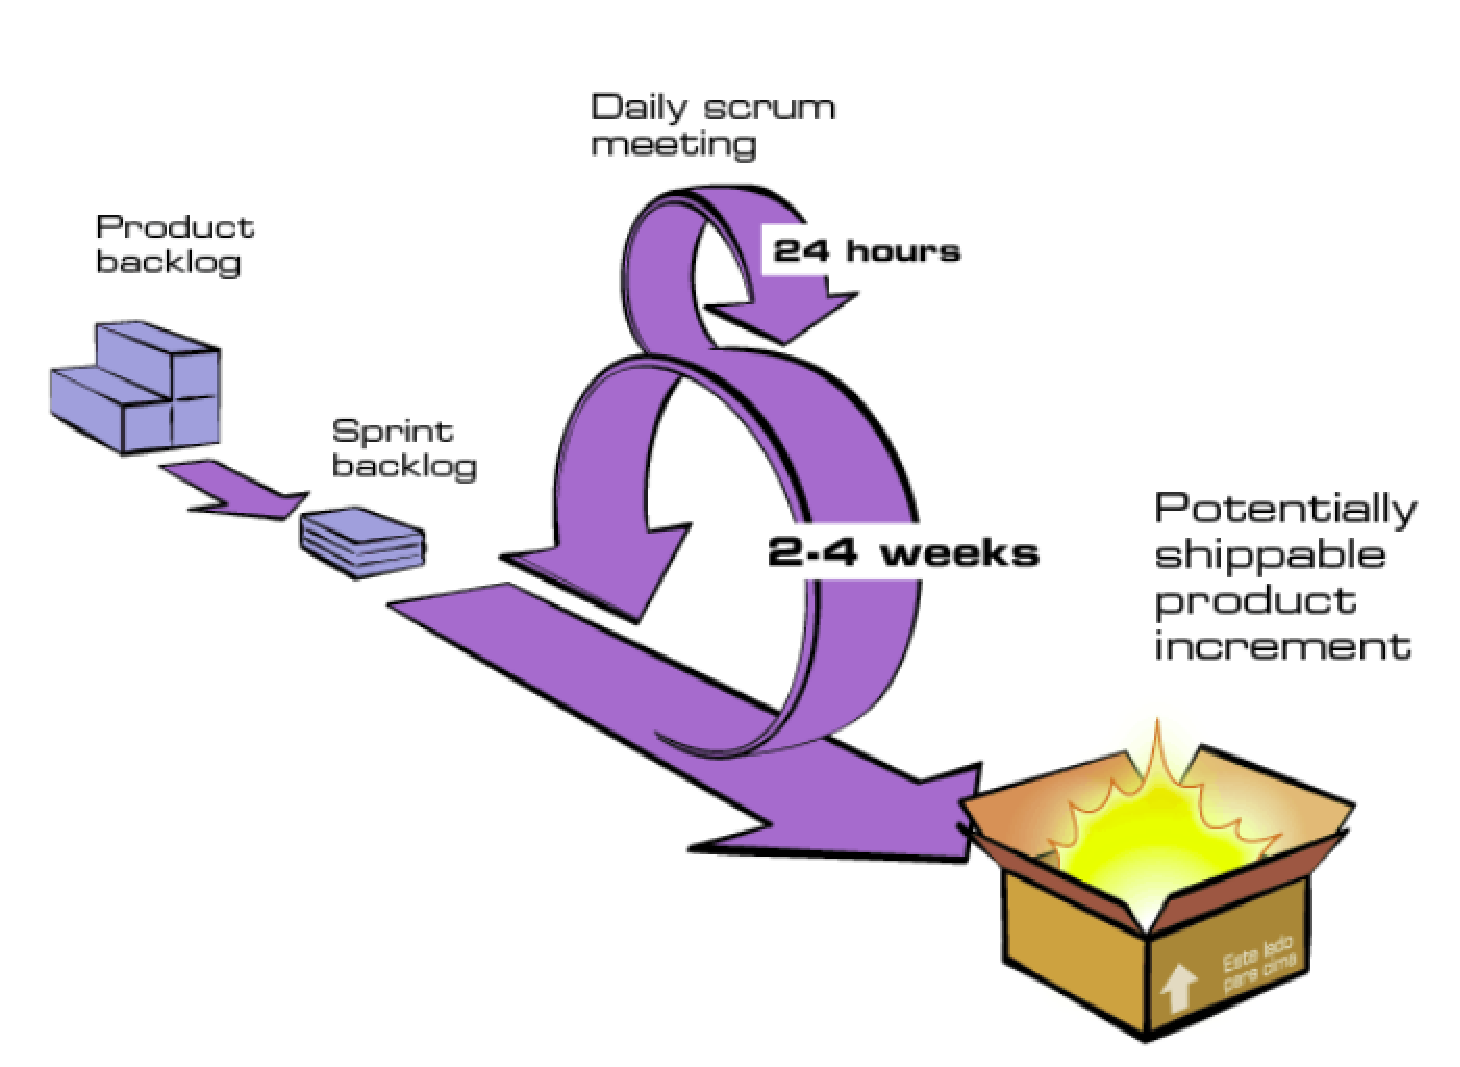
\includegraphics[keepaspectratio=true,scale=0.6]{figuras/scrum.eps}
  \caption[Processo iterativo do SCRUM.]{Processo iterativo do SCRUM. Fonte: \cite{diniz}}
	\label{fig:scrum}
\end{figure}

No capítulo 3 será mais detalhado como foi aplicado as atividades e artefatos dessa metodologia.

\subsection{XP}

\textit{Extreme Programming} ou XP é uma metodologia de desenvolvimento de software que ajuda a criar sistemas de melhor qualidade, que são produzidos em menos tempo e de forma mais econômica que o habitual. Tais objetivos são alcançados através de um pequeno conjunto de valores, princípios e práticas. \cite{beck}

\subsubsection{Valores}

De acordo com \cite{beck} para que as equipes sejam efetivas temos que seguir os seguintes valores:

\begin{itemize}
  \item \textbf{Comunicação}: A comunicação é essencial para o êxito da metodologia e pode ser realizada de diversas formas, não somente por documentação como nas metodologias tradicionais. A comunicação entre os desenvolvedores instiga a disseminação do conhecimento dentro da equipe, já a comunicação com o cliente garante que o produto entregue atenda à suas expectativas;
  \item \textbf{Feedback}: O feedback consiste que o programador terá informações constantes do código e do cliente.  Dessa forma, a equipe que está desenvolvendo o sistema tem uma visão clara acerca dos requisitos e do que é necessário que seja implementado;
  \item \textbf{Simplicidade}: Sempre que foi iniciado a implementação de algo, deve ser questionado qual a forma mais fácil de implementar aquele escopo, ou seja, não criar coisas desnecessárias ou que tenha uma complexidade alta;
  \item \textbf{Coragem}: É necessário coragem para implantar os três valores anteriores e consiste na coragem durante a implementação de tomar decisões que sejam melhores para a equipe e para o código. Por exemplo, refatorar códigos já implementados para garantir a qualidade do código.
\end{itemize}

\subsubsection{Práticas}

De acordo com \cite{beck} o XP baseia-se em 12 práticas a ser seguidas:

\begin{itemize}
  \item \textbf{Planejamento}: Decidir o que é necessário ser feito e o que pode ser adiado no projeto;
  \item \textbf{Entregas Frequentes}: Construção de pequenas funcionalidades conforme os requisitos surgem, ou seja, há sempre uma atualização do software. Cada versão entregue deve ter conter os requisitos de maior valor para o negócio. Idealmente devem ser entregues versões a cada mês, aumentando a possibilidade de feedback rápido do cliente;
  \item \textbf{Metáfora}: Descrições do software sem a utilização de termos técnicos;
  \item \textbf{Projeto Simples}: O programa deve ser o mais simples possível e satisfazer os requisitos atuais;
  \item \textbf{Propriedade Coletiva}: O código do projeto pertence a todos os membros da equipe, ou seja, codificar para o outro e não para si mesmo, fazendo de tudo para que o próximo que for mexer no código entenda o que está acontecendo. No XP todos são responsáveis pelo código inteiro;
  \item \textbf{Testes automatizados}: Teste é o processo de executar um programa ou sistema com a intenção de encontrar defeitos, entre os testes mais conhecidos estão os testes unitários que visa encontrar defeitos em pequenas unidades do software, testes de integração que busca encontrar defeitos na integração entre várias partes do software, testes de aceitação que busca encontrar defeitos nas interfaces do software e testes de regressão que busca encontrar defeitos que foram gerados por novas modificações;
  \item \textbf{Programação pareada}: É uma prática que sugere que o código seja sempre trabalhado em dupla em um mesmo computador, revezando quem está digitando;
  \item \textbf{Refatoração}: É o processo de reorganizar a estrutura interna do software, sem alterar seu comportamento externo, sempre pensando na qualidade do produto;
  \item \textbf{Integração contínua}: A integração contínua é a prática de manter a build sempre estável com novas funcionalidades, ela permite que seja executado testes antes das novas funcionalidades ser integrados no código que irá para o ambiente de produção, ou seja, o ambiente na qual o usuário irá utilizar o software. Isso permite construir confiança e garantir qualidade nas funcionalidades;
  \item \textbf{40 horas de trabalho semanal}:  A XP assume que não se deve fazer hora extra constantemente;
  \item \textbf{Cliente presente}: É muito importante a participação do cliente em todo o desenvolvimento do projeto;
  \item \textbf{Código padrão}: Padronização da arquitetura do código para que esse possa ser entendido por todos.
\end{itemize}

\subsection{SAFe}

A engenharia de requisitos é um conjunto de atividades utilizadas para identificar e comunicar a finalidade de um sistema de software, e o contexto no qual será usado \cite{leffingwell}.

O \textit{Scaled Agile Framework} ou SAFe é uma base de conhecimento on-line, de padrões de sucesso para pessoas que estão
construindo softwares e sistemas. Ele descreve as funções, responsabilidades, artefatos e atividades necessárias para
implementar o desenvolvimento ágil \cite{safe}

O SAFe permite que cada organização o adapte às suas próprias necessidades de negócios, ou seja, suporta soluções de menor escala bem como sistemas complexos.

Esse tópico irá abordar apenas a rastreabilidade de requisitos do SAFe que será utilizado no projeto. Essa
rastreabilidade no SAFe é organizada de forma hierárquica sempre diminuindo o nível de granularidade do requisito de
Tema de investimento até histórias de usuário e tarefas.

De acordo com \cite{safe} os temas associados a requisitos, se dividem, por fases:

\subsubsection{Fase de portfólio}

Fase responsável por alinhar estratégia de negócio e intenções de investimento, assim que a equipe tem a descrição do
valor, isso pode ser quebrado em funcionalidades menores que são chamadas de épicos, por exemplo, um tema de
investimento de um e-commerce tem como épicos, sistema de autenticação/autorização, sistema de vendas, catálogo de
produtos, entre outros. É nessa fase que é aplicado a engenharia de requisitos.

\subsubsection{Fase de programa}

Fase responsável pela auto-organização de times ágeis, entrega contínua de valor e criação de \textit{features} baseado nos épicos encontrados.

\subsubsection{Fase de time}

Fase responsável pelo auto-gerenciamento da equipe ágil, incremento do software totalmente testado, práticas \textit{SCRUM} e \textit{XP}, descrição do valor por meio de histórias de usuários e tarefas que são derivadas das \textit{features} encontradas na fase de programa.

